\documentclass[conference]{IEEEtran}
\usepackage{amsmath}          % Ecuaciones
\usepackage{amssymb}          % S�mbolos
\usepackage{hyperref}         % Vinculos 
\usepackage{graphicx}         % Graficos
\usepackage{graphics}         % Subfiguras
\usepackage[tight,footnotesize]{subfigure}

% *** CITATION PACKAGES ***
%
\usepackage{cite}
% cite.sty was written by Donald Arseneau
% V1.6 and later of IEEEtran pre-defines the format of the cite.sty package
% \cite{} output to follow that of IEEE. Loading the cite package will
% result in citation numbers being automatically sorted and properly
% "compressed/ranged". e.g., [1], [9], [2], [7], [5], [6] without using
% cite.sty will become [1], [2], [5]--[7], [9] using cite.sty. cite.sty's
% \cite will automatically add leading space, if needed. Use cite.sty's
% noadjust option (cite.sty V3.8 and later) if you want to turn this off.
% cite.sty is already installed on most LaTeX systems. Be sure and use
% version 4.0 (2003-05-27) and later if using hyperref.sty. cite.sty does
% not currently provide for hyperlinked citations.
% The latest version can be obtained at:
% http://www.ctan.org/tex-archive/macros/latex/contrib/cite/
% The documentation is contained in the cite.sty file itself.
% *** SPECIALIZED LIST PACKAGES ***
%
%\usepackage{algorithmic}
% algorithmic.sty was written by Peter Williams and Rogerio Brito.
% This package provides an algorithmic environment fo describing algorithms.
% You can use the algorithmic environment in-text or within a figure
% environment to provide for a floating algorithm. Do NOT use the algorithm
% floating environment provided by algorithm.sty (by the same authors) or
% algorithm2e.sty (by Christophe Fiorio) as IEEE does not use dedicated
% algorithm float types and packages that provide these will not provide
% correct IEEE style captions. The latest version and documentation of
% algorithmic.sty can be obtained at:
% http://www.ctan.org/tex-archive/macros/latex/contrib/algorithms/
% There is also a support site at:
% http://algorithms.berlios.de/index.html
% Also of interest may be the (relatively newer and more customizable)
% algorithmicx.sty package by Szasz Janos:
% http://www.ctan.org/tex-archive/macros/latex/contrib/algorithmicx/




% *** ALIGNMENT PACKAGES ***
%
%\usepackage{array}
% Frank Mittelbach's and David Carlisle's array.sty patches and improves
% the standard LaTeX2e array and tabular environments to provide better
% appearance and additional user controls. As the default LaTeX2e table
% generation code is lacking to the point of almost being broken with
% respect to the quality of the end results, all users are strongly
% advised to use an enhanced (at the very least that provided by array.sty)
% set of table tools. array.sty is already installed on most systems. The
% latest version and documentation can be obtained at:
% http://www.ctan.org/tex-archive/macros/latex/required/tools/


%\usepackage{mdwmath}
%\usepackage{mdwtab}
% Also highly recommended is Mark Wooding's extremely powerful MDW tools,
% especially mdwmath.sty and mdwtab.sty which are used to format equations
% and tables, respectively. The MDWtools set is already installed on most
% LaTeX systems. The lastest version and documentation is available at:
% http://www.ctan.org/tex-archive/macros/latex/contrib/mdwtools/


% IEEEtran contains the IEEEeqnarray family of commands that can be used to
% generate multiline equations as well as matrices, tables, etc., of high
% quality.


%\usepackage{eqparbox}
% Also of notable interest is Scott Pakin's eqparbox package for creating
% (automatically sized) equal width boxes - aka "natural width parboxes".
% Available at:
% http://www.ctan.org/tex-archive/macros/latex/contrib/eqparbox/





% *** SUBFIGURE PACKAGES ***
%\usepackage[tight,footnotesize]{subfigure}
% subfigure.sty was written by Steven Douglas Cochran. This package makes it
% easy to put subfigures in your figures. e.g., "Figure 1a and 1b". For IEEE
% work, it is a good idea to load it with the tight package option to reduce
% the amount of white space around the subfigures. subfigure.sty is already
% installed on most LaTeX systems. The latest version and documentation can
% be obtained at:
% http://www.ctan.org/tex-archive/obsolete/macros/latex/contrib/subfigure/
% subfigure.sty has been superceeded by subfig.sty.



%\usepackage[caption=false]{caption}
%\usepackage[font=footnotesize]{subfig}
% subfig.sty, also written by Steven Douglas Cochran, is the modern
% replacement for subfigure.sty. However, subfig.sty requires and
% automatically loads Axel Sommerfeldt's caption.sty which will override
% IEEEtran.cls handling of captions and this will result in nonIEEE style
% figure/table captions. To prevent this problem, be sure and preload
% caption.sty with its "caption=false" package option. This is will preserve
% IEEEtran.cls handing of captions. Version 1.3 (2005/06/28) and later 
% (recommended due to many improvements over 1.2) of subfig.sty supports
% the caption=false option directly:
%\usepackage[caption=false,font=footnotesize]{subfig}
%
% The latest version and documentation can be obtained at:
% http://www.ctan.org/tex-archive/macros/latex/contrib/subfig/
% The latest version and documentation of caption.sty can be obtained at:
% http://www.ctan.org/tex-archive/macros/latex/contrib/caption/




% *** FLOAT PACKAGES ***
%
%\usepackage{fixltx2e}
% fixltx2e, the successor to the earlier fix2col.sty, was written by
% Frank Mittelbach and David Carlisle. This package corrects a few problems
% in the LaTeX2e kernel, the most notable of which is that in current
% LaTeX2e releases, the ordering of single and double column floats is not
% guaranteed to be preserved. Thus, an unpatched LaTeX2e can allow a
% single column figure to be placed prior to an earlier double column
% figure. The latest version and documentation can be found at:
% http://www.ctan.org/tex-archive/macros/latex/base/



%\usepackage{stfloats}
% stfloats.sty was written by Sigitas Tolusis. This package gives LaTeX2e
% the ability to do double column floats at the bottom of the page as well
% as the top. (e.g., "\begin{figure*}[!b]" is not normally possible in
% LaTeX2e). It also provides a command:
%\fnbelowfloat
% to enable the placement of footnotes below bottom floats (the standard
% LaTeX2e kernel puts them above bottom floats). This is an invasive package
% which rewrites many portions of the LaTeX2e float routines. It may not work
% with other packages that modify the LaTeX2e float routines. The latest
% version and documentation can be obtained at:
% http://www.ctan.org/tex-archive/macros/latex/contrib/sttools/
% Documentation is contained in the stfloats.sty comments as well as in the
% presfull.pdf file. Do not use the stfloats baselinefloat ability as IEEE
% does not allow \baselineskip to stretch. Authors submitting work to the
% IEEE should note that IEEE rarely uses double column equations and
% that authors should try to avoid such use. Do not be tempted to use the
% cuted.sty or midfloat.sty packages (also by Sigitas Tolusis) as IEEE does
% not format its papers in such ways.





% *** PDF, URL AND HYPERLINK PACKAGES ***
%
%\usepackage{url}
% url.sty was written by Donald Arseneau. It provides better support for
% handling and breaking URLs. url.sty is already installed on most LaTeX
% systems. The latest version can be obtained at:
% http://www.ctan.org/tex-archive/macros/latex/contrib/misc/
% Read the url.sty source comments for usage information. Basically,
% \url{my_url_here}.





% *** Do not adjust lengths that control margins, column widths, etc. ***
% *** Do not use packages that alter fonts (such as pslatex).         ***
% There should be no need to do such things with IEEEtran.cls V1.6 and later.
% (Unless specifically asked to do so by the journal or conference you plan
% to submit to, of course. )


% correct bad hyphenation here
\hyphenation{op-tical net-works semi-conduc-tor}
\hyphenation{ener-gy}
\hyphenation{po-we-red}

\begin{document}
\hypersetup{pdfborder=0 0 0}
% paper title
% can use linebreaks \\ within to get better formatting as desired
\title{Design and implementation of a Lunabot using NASA Systems Engineering}


% author names and affiliations
% use a multiple column layout for up to three different
% affiliations
\author{\IEEEauthorblockN{Johan Sebastian Macias, Jorge Mario Garzon Rey, Camila Andrea Gonzalez, Carlos Edinson Roso, \\
Juan Sebastian Velandia, Juan Pablo Barreto, Nicolas Ochoa, Carlos Francisco Rodriguez, Antonio Garcia-Rozo}
\IEEEauthorblockA{Department of Electrical and Electronics Engineering \\Department of Mechanical Engineering\\
Universidad de los Andes\\
Bogota D.C., Colombia\\
Email:\{js.macias121,pa-barre,n-ochoa,crodrigu,angarcia\}@uniandes.edu.co}
}
 
%jm.garzon131,ca.gonzalez961,a.latorre70,ce.roso398,js.velandia157
% make the title area
\maketitle


\begin{abstract} %(JMGR)
This paper presents  the design, construction, verification, and validation process of a Lunar Excavation Prototype (Lunabot) under NASA Systems Engineering guidelines followed by Robocol Team for the Third NASA Lunabotics Mining Competition. The systems engineering approach highly applied in NASA's projects, proposes an organization through phases to ensure a successful product, answering the problem stated. The program formulation is composed by several phases which general goal is to list all the requirements of the project from the technical specifications to the budget for his development. 
\end{abstract}

\begin{IEEEkeywords}
NASA Systems Engineering, Lunar Excavation Prototype, Regolith.
\end{IEEEkeywords}

\IEEEpeerreviewmaketitle

\section{Introduction}%(JMGR)

Third Lunabotics Mining Competition  is an international contest held by NASA which encourages teams to get involved in lunar exploration, by building a robot, called Lunabot, that shall collect the maximum lunar regolith simulant in the minimum time. This document illustrates the design, construction, verification, and validation process of a Lunar Excavation Prototype (Lunabot) under NASA Systems Engineering guidelines \cite{NASASysEng1995} followed by Robocol  for the Lunabotics Competition.

There are two major expectations within the development of a lunabotics Project hosted by NASA. Promote the development of interest in space activities and STEM (Science, Technology, Engineering, and Mathematics), and focus this interest in a novel approach for tackling complex technical challenges that has gained popularity in recent years. Through this, a sponsoring company holds a contest in which a similar challenge is proposed, resulting in interesting concepts that could actually function under real conditions \cite{NASArules2012}.

Fuel and oxygen are two imperative needs for human manned missions on the moon, and furthermore for coming lunar stations.  Particularly in this project, the challenge of designing, building and testing a robot, which its main objective is to excavate and transport lunar regolith is a priority for mentioned activities on the moon. Basically because evidence shows that lunar soil has significant amount of both oxygen~\cite{wiechert2001oxy} and fuel~\cite{Wittenberg1986}. 

Robocol  team is constituted by eleven Mechanical Engineering undergraduate students, nine Electronics Engineer undergraduate students, two Industrial Engineering undergraduate students, one Design undergraduate students, three  advisers from the Mechanical Engineering Department and one advisor form Department of Electrical and Electronics Engineering.

As the main feature for Lunabotics Mining competition, Robocol´s participating Lunabot  is presented in Figure~\ref{fg: fig1}.  The following sections describe the design fabrication and verification process to achieve this robot. 

\begin{figure}[!tbh] 
 \centering
 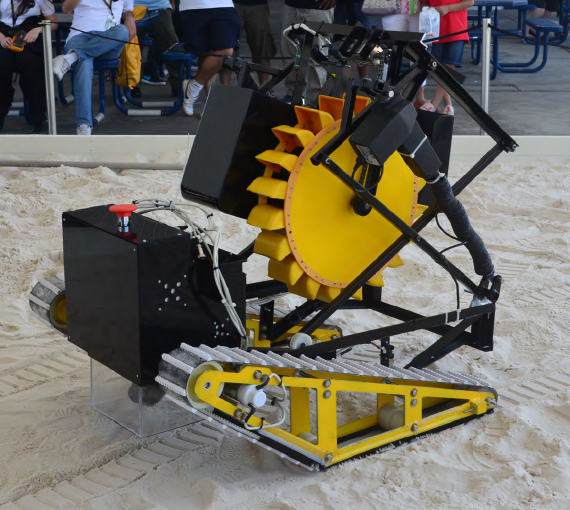
\includegraphics
 [width=0.8\linewidth]{img/Figure1}
 \caption{Robocol's lunabot up to date}
 \label{fg: fig1}
 \end{figure}

% Hipotesis:  Utilizar INg SIS para luanbot
\section{NASA Systems Engineering} % (JMGR - VELANDIA)

The systems engineering approach is a useful tool for any design process. This method, highly applied in NASA's projects, proposes an organization through phases to ensure a successful product, answering the problem stated. All the phases described by the method can be classified in two main activities: Formulation and Implementation. 

The program formulation is composed by several phases which general goal is to list all the requirements of the project from the technical specifications to the budget for his development. Two phases are distinguished in this part of the project.

The phase A and its preparation is supposed to include the analysis and evaluation of all the ideas proposed to solve the problem. The final task in this stage is to have enough simulations, models and even rough prototypes to choose the right concept to develop.

The phase B uses the concepts defined in the previous phase and converts it into a final product, filling all the requirements stated. This phase ends not only with the concept of the solution defined but also with an analyzed and simulated prototype of the product able to accomplish its mission.

After the program formulation, the program implementation is the next big step, it is supposed to lead the process as stated the phase B. This part of the project focuses on fabricating, assembling, testing and operating the solution. Four phases are detected during the implementation.

The phase C is the last step, of the solution's design and the first of its production. In this phase, the project team verifies the structure of the design, the details in sub-systems and systems, the way they are going to be assembled. As a result, a final design is produced, and most of the components are fabricated.

As expected, phase D is the assembly of systems with all the tests required. Nevertheless, the assembly of sub-systems is not enough to reach the desired system; an integration process has to be done through this phase. Finally, 	the product is ready to begin its operation.

Phases E and F are focused on the performance of the product. This phases work with the desired system in the operating conditions and trying to achieve the goal it was designed for

As a result of the application of this method, NASA has produced rovers, space shuttles and rockets. All processes in NASA follow this guideline. The process described here generate a workflow during the project ensuring an structured result.


\section{Methodology}

\subsection{Phase A}
It was required to build a lunabot as light as possible, which must Excavate at least 10 kg of regolith, controlled remotedly via wifi, with protection for dust tolerant operation, energy consumption report, low data transmission and partial or total autonomy. 

For the mechanical system there were identified three subsystems: Excavation, Traction, Discharge.

The main target of the  Excavation  was avoid loss of regolith and increasing efficiency. The requirement of lightweight mechanism was included.  Two solutions were proposed for this system, a screw conveyor and a bucket with a ramp. The bucket wheel achieves a better excavation rate of 80g/s vs. 60g/s of the screw conveyor. The best option for the excavation system is the bucket wheel and ramp system, it is the starting point for the final system design. 

The Traction system objective was to be as quick and lightweight as the 4$ \times $4 system, but it had to ensure a good maneuverability. Two solutions were proposed as well; an ackerman steering mechanism, and a vehicle driven by crawlers. The Ackerman steering mechanism has a lower power demand; it is also lighter than crawlers, which penalizes the power consumption comparison. A first impression would be that this system is more adequate than the crawlers; nevertheless structural integrity, stability, and the ability to support other structures make the crawlers a better choice. 


Regarding the discharge system, a great uncertainty was present in the rest angle of the regolith.  This implied overdesigned slopes in the containers or discharge mechanisms, and the use of vibrators for improved sliding of the regolith. A rigorous study on regolith properties was performed to reduce the uncertainty. 

The amount created seemed enough to understand BP-1 behavior in storage and discharge system but it is not enough to test mining or transport systems.  At this time evaluations are held to determine if it is worthy to continue creating BP-1 simulant to test all Lunabot's systems. 

Acknowledging that the container in which regolith must be deposited is over 50 cm the probability of needing a lifting mechanism is high if a stable robot is desired. The scissors mechanism is highly recommended for this purpose because proved being reliable, lightweight and demanded acceptable power levels.

By the other hand, size and shape of a provisional container were designed and built. Container was restricted to a volume of 80cm~$\times$~16cm~$\times$~40cm. Due to the lifting system, a rectangle shaped container was not the best choice; a high angle on the discharge side was needed to ensure that all the regolith excavated would be able to leave the container. Kinematic analysis (and further test) proved that, if the container started in horizontal position, scissors system achieved an inclination angle of 25$^\circ $, which did not seem enough to ensure desired condition. The inclination angle was improved on 27$^\circ $.

For the electronics system there were identified five subsystems: Control and Data processing, Comunication, Sensing and Power and energy supply.

The target of the Power and energy supply subsystem was designing and implementing the circuitry for receiving digital signals from the Control Subsystem and traducing them into high current analog signals to power the traction and digging motors as well as the linear actuators. Also, this subsystem had the task of suplying all the energy required by the entire Lunabot. For the circuitry to power the motors two options were taken into account: An H bridge and a driver implemented with discrete components available in the local market in Colombia, and a fully integrated monolithic Hbridge motor driver (VNH3ASP30). For the circuitry to power the linear actuators, the use of relays  was considered, based on the experience of  the last year competition. For the energy supply it was considered the use of 5000mAh @12V LiPo batteries for motor supply and to use a 5000mAh @24V battery for the two linear actuators.

The objective of the Sensing subsystem was the recognition of holes and obstacles, the detection of regolith mass in the container and the image acquisition.  For the recognition of holes and obstacles capacitive and inductive sensors as well as infrared sensors were evaluated. Regarding to the detection of regolith mass in the container  it was considered to place infrared sensors inside the container as well as using limit switches to mark a set of discrete levels of regolith in the container. For the images acquisition there were contemplated single and dual RGB cameras, a Laser Range-Finder and the Microsoft Kinect (IR+ RGB pair)

The Control and Data Procession subsystem was intented to receive process and send the digital signals to control remotedly, semiatonomously or autonomously the Lunabot. Regarding to the central control unit, two ideas where proposed: Using a netbook (Toshiba NB255) or an industrial embedded computer (Advantech PCM-3363D-1GS8A1E).  Both options where analized and compared in terms of memory, weight, procesor, ports and power suppy. 

For the purpose of performing Input/Output operations between the central control unit and the hardware of the Lunabot (i.e. H-bridge drivers for the motors, the relay board for the linear actuators, the distance sensors, etc.) it was required a device to process the required analog and digital signals. Two options were contemplated:  using a dsPIC30F4011 for PWM signal generation and an ATxmega32A4 microcontroller for acquisition of data from sensors or employing two Arduino Mega Boards (one for motor control and the other for control of actuators and acquisition of sensors).

To achieve the autonomous and semiautonomous operation three main goals were established: Identify obstacles and planes, identify a fixed beacon and determine a navigation path through the Lunarena.

The Communication subsystem involved the implementation of a user interface to remotely operate the Lunabot from a Control Computer; the implementation of a script to handle the data flow transmitted and received between the Control Computer wireless adapter and the Lunabot; and the use of a wireless device in the Lunabot to transmit and receive the data. Concerning the implementation of the user interface and the script for the data flow handling, it was considered to use Python 2.7. For the wireless device, it was contemplated the use of a Lantronix MatchPort b/g embedded.

\subsection{Phase B}
\subsection{Hierarchy  of designed Systems }

Figure~\ref{fg: fig19} shows the hierarchy established for the mechanical systems. In it, the first level is recognized as the structure or chassis, every other part or mechanism is attached to it, or to other systems that are joined to the chassis. Then, in the second level the traction system and the lifting system are allocated because once they are joined to the structure, they perform their functions. On the third level there  is located the excavation and discharge system because they perform their function only when they are joined to the lifting system.

 \begin{figure}[!htb] 
 \centering
 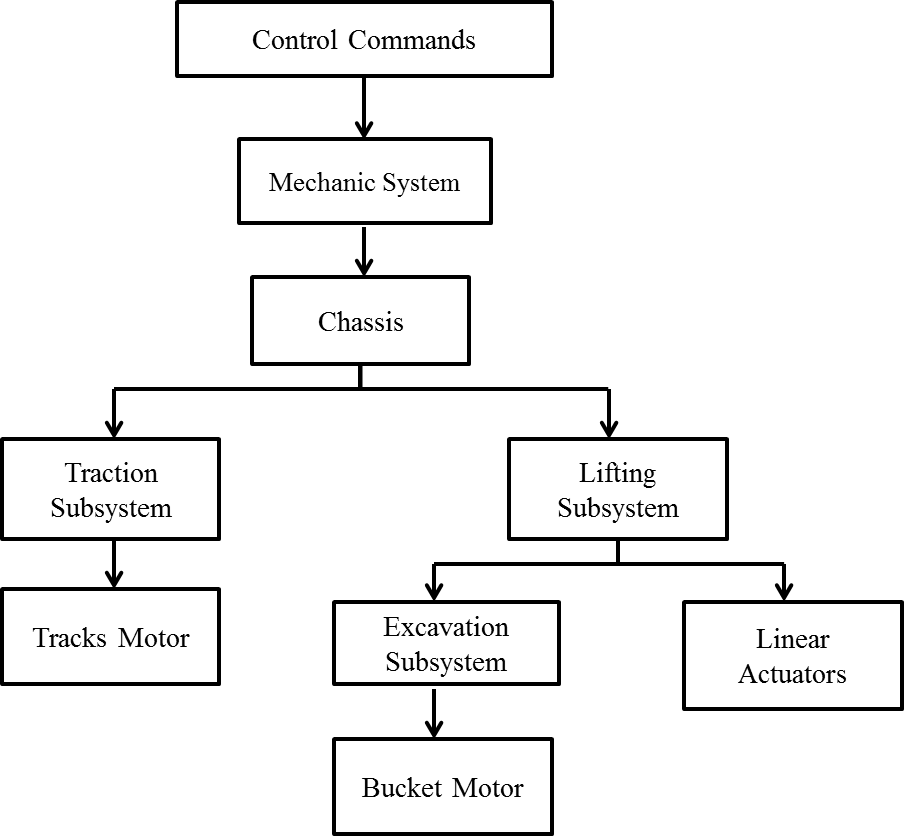
\includegraphics [width=0.8\linewidth]{img/Figure20}
 \caption{Hierarchy of mechanical systems}
 \label{fg: fig19}
 \end{figure}

Once the hierarchy diagram has been developed for mechanical and electronic systems, Figure~\ref{fg: fig20} presents de hierarchy diagram for the whole robot taking into account all systems.

 \begin{figure*}[!htb] 
 \centering
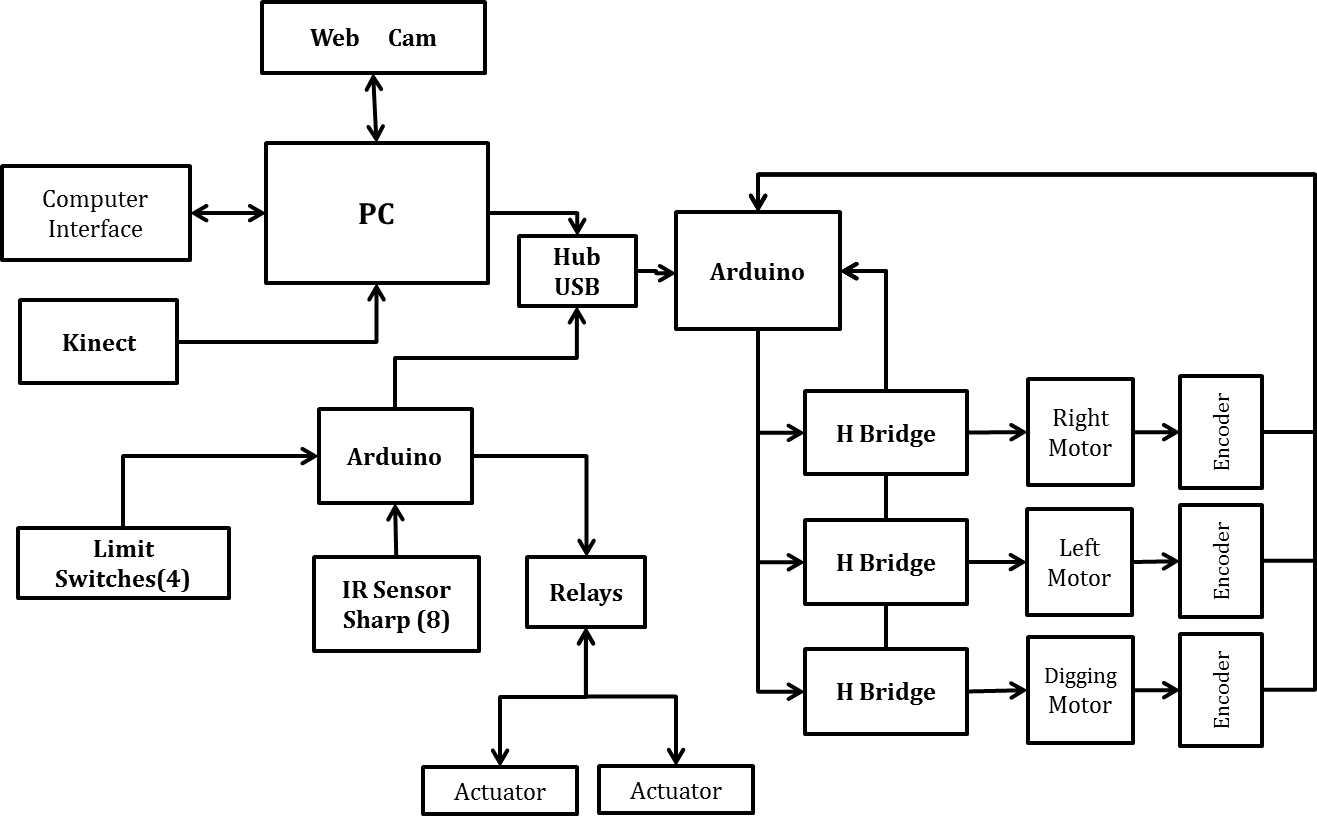
\includegraphics [width=0.8\linewidth]{img/Figure20e}
 \caption{Block diagram} 
 \label{fg: fig20}
 \end{figure*}

The control system receives commands from the user through the communication subsystem. It then transforms these commands into digital signals to move the motors and the actuators and send them to the power subsystem. Also, the control receives the data sensed from the sensing subsystem, processes it, and sends these data to the control computer if it is requested.

The diagram Shown in  Figure~\ref{fg: fig20} details a description of the electronic system.  As shown, the Netbook sends and receives directly the signals from the user interface. It also receives the images from the Web Camera and the Kinect sensor. In addition, two Arduinos are used for the Control and Processing System. One of them is used to send PWM signals, through the H-Bridge, to the traction and excavation motors; also it is used to process the motors’ current sensed by the H-Bridges as well as the motors’ position as marked by the encoders. The other Arduino is used to send control signals to the linear Actuators through the relays’ control circuitry; It is also used to process the signals from the Sharp IR Sensors and from the limit switch sensors. 

In the final design of the electronics subsystem it was decided to use the Netbook as the central controller and processing unit in the Lunabot and using the arduino platform because it reduces the programing, uploading and testing time in the prototyping cycle. The Arduino platform is an open source project for fast prototyping of electronic systems. 
For the acquisition of images it was decided to use a Kinect Sensor as the main device for images acquisition, and a simple Web Camera as an auxiliary sensor.
For the user interface it was decided to use phython , due to its unique mix of features: it is open source, it has an ample codebase of libraries and it has a large and active community.

Two modular crawlers compose traction system chosen. Each crawler has its own aluminum structure where motor and rollers are assembled. The triangular shape of the structure allows the motor to be far from traction area, reducing its failure by crash probability. Due to this separation, a chain-sprocket system is used to power transmission with a relation of 2:1, increasing system’s speed. 

Three subsystems compose the Lunabot’s excavation system: a bucket-wheel, an Archimede’s screw, an U-shaped canal with its corresponding drive shaft (with its sprocket).

The bucket wheel is composed by a 48cm diameter support were 20 buckets are assembly. Once the wheel is turning, excavated soil falls into the canal and is transported by the screw to the container.

Selection of the motor for this system is supported by similarity laws analysis done with a smaller bucket wheel. The result of the analysis shows that the motor selected for the traction system has enough torque to excavate the BP-1.

The discharge system is a passive door pivoted system, This system is composed by a container (72cm~$ \times $~23cm~$ \times $~15cm) and a small sheet (20cm) assembled by a hinge joint. A lifting system was required too, it was designed to lift and turn the container in order to guarantee the correct discharge of regolith.

Nevertheless, the shape of the container and its turning were not enough to guarantee this process, an additional metal sheet was assembled with a hinge.


\subsection{Phase C}
Detailed design of Subsystems was developed simultaneously by three groups of students who were the responsible of its subsequent manufacture. Process design of final version of the LUNABOT UNIANDES took two months between November 19 to January 19, and it involved the develop of relations  between the subsystems and all its specifications.

Mining subsystem design involved specifications of the manufacture blueprints of the bucket wheel and the regolith container of the robot and its relations with the elevation and chassis subsystems.

Mobility system design engaged specification of blueprints of the tracks and its relations with the chassis subsystem and fixing of its engines.

Appropriate elevation and chassis subsystems design were very important in the success of the entire robot, because these subsystems were the link between others, and it alloyed the excavation and the regolith discharge.  This design took in mind the use of two actuators and the strength of materials used.

Manufacture of each subsystem elements were carried out by students and technical personal of laboratories from university. It process took two months since January 19 to March 19. Some pieces needed specially manufacture, as regolith container made of fiber glass. These pieces were fabricated by Colombian companies based on the blueprints designed previously.


The electronic system was designed to accomplish several tasks such as driving the excavation and tracks motors, driving the linear actuators, acquiring signals from the sensors, … The central control of the whole system was a Netbook Toshiba NB255. It was connected via Wifi to the command center in order to send or receive data. Two Arduino boards (Mega) were plugged into the PC. One of them controlled the 3 motors and received the encoder signals from each one of these. The other one controlled the linear actuators and processed the signals from some sensors (limit switches and IR Sharp sensors). H bridge power drivers were implemented to drive the 30A motors. Both 2A linear actuators were driven from a relay based power driver. 


A client-server application was coded in Python 2.7 to control the robot from the command center. The server was deployed on the Netbook and the client was running on other PC located at the command center. Both Arduino boards were programmed in this phase as well. 

A fully integrated monolithic H Bridge motor driver was used to drive each one of the motors. Each driver was soldered in a PCB. Also, it was designed a PCB for each of the Arduino Board and for the linear actuators’ driver. Each PCB was designed to be connected into a 50 pins edge connector. A COTS red button was used for the emergency stop; however, a high current relay board was designed to power the whole system off.


\subsection{Phase D}
The assembly process took one month, since March 19 to April 19, and involves the Integration of all mechanical subsystems and the electronic system.

Integration tests were developed since April 19 to May 15, and it involved testing of mobility, excavation, regolith discharge and obstacle avoid capability. These testing process were performed at sandpit of the project located in COLIVRY laboratory from UNIANDES.

Shipping of robot was developed by subsystems packed in different boxes and shipped like luggage in the fly of the team members.

Due to the considerable amount of connections between all the PCBs, it was appropriate to design a simple way to accomplish this task in an effective manner. Thus, a motherboard was design with a set of six 50 pin edge connectors to hold each PCB. All the connections were routed in the motherboard and each PCB was easily connected into the edge connectors. 

Six 12V LiPo batteries were used to power the whole system and a 24V LiPo battery was used for the linear actuators. 5V and 3.3V were obtained by regulating the voltage wherever needed. 

The hard drive was taken off the Netbook to avoid severe damages and an SD was used to boot the system and scripts. Both Arduino boards were powered and controlled by the Netbook.

Special wiring was considered to connect the sensors, motors and actuators to the electronic system. It was used a shielded wire to connect the IR Sharp sensors, while high current cables were used to power the motors and the actuators.

12V fans were located strategically to cool critical components. Finally, the red button and its relay board were connected to each subsystem respectively to power it on or off. Once the electronic system was fully assembled, it was ready to be tested.

The whole system was first powered on. The wireless connection between the command computer and the Netbook inside the robot was tested. All the commands were received properly by the Netbook. Also, both Arduino boards received the orders properly. Each H Bridge was tested for each motor and all of them worked properly. Due to the high currents involved in this test, some H Bridges got burned. However, the designers added some protections to the circuits and it finally worked. The motors worked properly with and without load. However, there was a high frequency sound that could be heard coming out from the motors due to the PWM signal. Despite this, the motors worked fine and managed to move the robot. The linear actuators worked properly as well.

Sensors signals seemed to be weak due to the relatively long distance to the electronic system. However, this fact did not have critical effects on the calibration of the sensors. High current cables did not get dramatically hot and managed to conduct the current properly. Finally, the red button was tested and the whole system was shut down including the Netbook (script coming from one Arduino).

\subsection{Phase E and F}

On Second  Lunabotics Mining Competition edition, 5 mechanical engineers and 1 electronic engineer formed the team. They had a good performance in the competition, placing 20th within 36 teams in the Joe Cosmo award of excellence without scoring in mining category. They achieved good scores in the Outreach Project and the Slide Presentation. Being a small group with major mechanical emphasis had as a consequence on the development of the project some issues due to the lack of work force in electronics area. For 2012, with the deep desire of improving 2011 representation, Robocol did some scouting labor, re-structured the team, and a strategic plan was developed, as shown above.

A remarkable fact that influences the project for phase A is that its starting point is located on the Lunabot presented for LMC 2011. Objectives proposed in phase A, came out partially from analyzing 2011 Lunabot performance, strengths and weaknesses. 

Figure~\ref{fg: fig 8} shows the Lunabot presented for 2011 LMC, two separated vehicles composed the Lunabot, the first  one, was indtended to excavate and the other one, to transport. This robot lied on the idea that a quick transportation needs lightweight hardware. On the other hand, a massive excavation demands big and robust structures.  In order to gain the advantages of a quick transportation, and abundant excavated mass, two vehicles, each one with demanded characteristics to comply quick transportation, and high excavation rates was presented.

 
  \begin{figure}[!htb] 
  \centering
  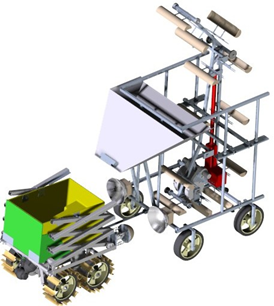
\includegraphics
  [width=0.6\linewidth]{img/Figure8}
  \caption{2011 Robocol's Lunabot}
  \label{fg: fig 8}
  \end{figure}
 
 
 One enormous difference between 2012 and 2011 LMC is the scoring system established for mining category. A main consequence is that the excavated mass is no longer the only variable which evaluates robot's performance.  In order to establish the main objectives according to scoring system, a sensibility analysis was executed.
 
 As a conclusion, according to the scoring system and technical difficulty, the team priorities are: To build a lunabot as light as possible, which must excavate 10 kg of regolith, with at least partial autonomy. The second level of priority would be: Improving excavated mass above 10 kg, and provide protection for dust tolerant operation. A third level is stated as full autonomy, energy consumption report, and low data transmission. The lunabot's mass becomes  five times more important than excavated mass. Acknowledging this fact, Robocol's team objective is to build a robot that is able to overpass -300 lunapoints, considering its weight and the excavated mass. Table~\ref{tb: score} shown the results for the 2012 Robocol Team participation.
 
 \begin{table}
 \centering
   \caption{Robocol Lunapoints}
     \begin{tabular}{rcc}
     \hline \hline
           & 1 Round & 2 Round \\
     \hline
     Pass Inspections & 1000  & 1000 \\
     Regolith over 10 kg & 0     & 0 \\
     Average Bandwidth & -2    & -2 \\
     Lunabot Mass & 450   & 460 \\
     Report Energy Consumed & 100   & 100 \\
     Dust Tolerant Design & 160   & 190 \\
     Full Autonomy & 0     & 0 \\
    \hline \hline
     \end{tabular}
   \label{tb: score}
 \end{table}


\section{Conclusions and Future Works} % CAmila
A systems-engineering driven approach to the design and construction of the Lunabot as been undergone. It has enabled the team adopt a strict and formal work flow in order to fulfill all stakeholder and subsequent derived requirements, so as to maximize the probability of mission success at the contest. The design process has been heavily influenced by the constraints imposed by the availability of components in the local market, as well as the technical characteristics of our Institution's facilities. We are still in the end of the testing processes, but remain confident the hard work undertaken for the sake of an ordered and structured development will yield the expected and long-awaited results.

The structured process over  10 months involved not only team members but also a lot of people through academic courses in the Universidad de los Andes. This cooperation allowed them to participate in Phase A, by proposing their own ideas, producing prototypes and learning from robotics principles and helped Robocol to decide its final design. Thanks to their experience, last year participants involved in the team enriched the entire process, their problems and success from last year were the starting point for many of the systems tested and selected this year. 

Since the entire process was done rigorously, good results were obtained in  Lunabotics Mining Competition 2012. However the objectives of excavating and depositing at least 10 kg of regolith during official attempt sessions were not successfully.  Robocol team had a good performance in the competition, placing 9th within 54 teams in the Joe Kosmo award of excellence without scoring in mining category.

\section*{Acknowledgment} 
The authors would like to acknowledge to Andres Latorre,  Fabio Lopez, Sebastian Ruiz, Santiago Grass,
Ramiro Montufar, Juan Felipe Moreno, Camilo Acosta, Christian Meneses, Franz Mojica, Luis Linares, Alvaro Gonzalez
Alejandro Montoya, Daniel Rodriguez, Sergio Bacca, John Estupiñan, Juan Camilo Machado, Andres Diaz  and Sergio Andres Moreno members of Robocol Team. and Also  to  the Printed Circuit Board laboratory and  Manufacturer laboratory staff  at Universidad de Los Andes for their support. 


% can use a bibliography generated by BibTeX as a .bbl file
% BibTeX documentation can be easily obtained at:
% http://www.ctan.org/tex-archive/biblio/bibtex/contrib/doc/
% The IEEEtran BibTeX style support page is at:
% http://www.michaelshell.org/tex/ieeetran/bibtex/
\bibliographystyle{IEEEtran}
% argument is your BibTeX string definitions and bibliography database(s)
\bibliography{IEEEabrv,references}

\end{document}

 
 \begin{figure}[!htb]
 \centering
 \includegraphics[width=0.7\linewidth]{img/DB_RX}
 \caption{Reader unit block diagram }
 \label{fg: DB_RX}
 \end{figure}
 
 % An example of a floating figure using the graphicx package.
 % Note that \label must occur AFTER (or within) \caption.
 % For figures, \caption should occur after the \includegraphics.
 % Note that IEEEtran v1.7 and later has special internal code that
 % is designed to preserve the operation of \label within \caption
 % even when the captionsoff option is in effect. However, because
 % of issues like this, it may be the safest practice to put all your
 % \label just after \caption rather than within \caption{}.
 %
 % Reminder: the "draftcls" or "draftclsnofoot", not "draft", class
 % option should be used if it is desired that the figures are to be
 % displayed while in draft mode.
 %
 %\begin{figure}[!t]
 %\centering
 %\includegraphics[width=2.5in]{myfigure}
 % where an .eps filename suffix will be assumed under latex, 
 % and a .pdf suffix will be assumed for pdflatex; or what has been declared
 % via \DeclareGraphicsExtensions.
 %\caption{Simulation Results}
 %\label{fig_sim}
 %\end{figure}
 
 % Note that IEEE typically puts floats only at the top, even when this
 % results in a large percentage of a column being occupied by floats.
 
 
 % An example of a double column floating figure using two subfigures.
 % (The subfig.sty package must be loaded for this to work.)
 % The subfigure \label commands are set within each subfloat command, the
 % \label for the overall figure must come after \caption.
 % \hfil must be used as a separator to get equal spacing.
 % The subfigure.sty package works much the same way, except \subfigure is
 % used instead of \subfloat.
 %
 %\begin{figure*}[!t]
 %\centerline{\subfloat[Case I]\includegraphics[width=2.5in]{subfigcase1}%
 %\label{fig_first_case}}
 %\hfil
 %\subfloat[Case II]{\includegraphics[width=2.5in]{subfigcase2}%
 %\label{fig_second_case}}}
 %\caption{Simulation results}
 %\label{fig_sim}
 %\end{figure*}
 %
 % Note that often IEEE papers with subfigures do not employ subfigure
 % captions (using the optional argument to \subfloat), but instead will
 % reference/describe all of them (a), (b), etc., within the main caption.
 
 
 % An example of a floating table. Note that, for IEEE style tables, the 
 % \caption command should come BEFORE the table. Table text will default to
 % \footnotesize as IEEE normally uses this smaller font for tables.
 % The \label must come after \caption as always.
 %
 %\begin{table}[!t]
 %% increase table row spacing, adjust to taste
 %\renewcommand{\arraystretch}{1.3}
 % if using array.sty, it might be a good idea to tweak the value of
 % \extrarowheight as needed to properly center the text within the cells
 %\caption{An Example of a Table}
 %\label{table_example}
 %\centering
 %% Some packages, such as MDW tools, offer better commands for making tables
 %% than the plain LaTeX2e tabular which is used here.
 %\begin{tabular}{|c||c|}
 %\hline
 %One & Two\\
 %\hline
 %Three & Four\\
 %\hline
 %\end{tabular}
 %\end{table}
 
 
